コースの幅が5つあり,それぞれの幅で十回(毎回8分間)実験する,一実験毎に,ランダムにロボットを2つグループを分ける.$T_{\rm 1d}$と流量($Q$)を計測して,平均値と標準偏差を計算する.
%\begin{table}[!ht]
%\setlength\tabcolsep{1pt}
%\begin{center}
%\begin{tabular}{|c|c|c|c|c|}
%\hline
%幅& $\bar{T}_{\rm 1d}$ & $s_{T_{\rm 1d}}$ & $\bar Q$ & $s_Q$ \\
%($m$)   &  (分) & 標本標準偏差 & 台/$ m\cdot min$ & 標準偏差 \\
%\hline
%0.430 & 8.00 & 0 & 0.44 & 0.15 \\
%\hline
%0.495 & 6.57 & 2.28 & 3.22 & 2.81 \\
%\hline
%0.560 & 4.63 & 2.23 & 5.25 & 3.39 \\
%\hline
%0.625 & 4.57 & 1.78 & 3.29 & 2.77 \\
%\hline
%0.690 & 4.56 & 2.32 & 5.41 & 3.50 \\
%\hline
%\end{tabular}
%\end{center}
%\caption{
%幅により$T_{\rm 1d}$と流量の値
%}
%\end{table} 
図\ref{dia1}はコース幅($w$)による,$T_{\rm 1d}$平均値の変化曲線である.図\ref{dia2}がコース幅による,平均流量($Q$)の変化曲線である.
オレンジ色の縦線はエラーバーである

\vspace{-1mm}
\begin{figure}[!ht]
    \centering
    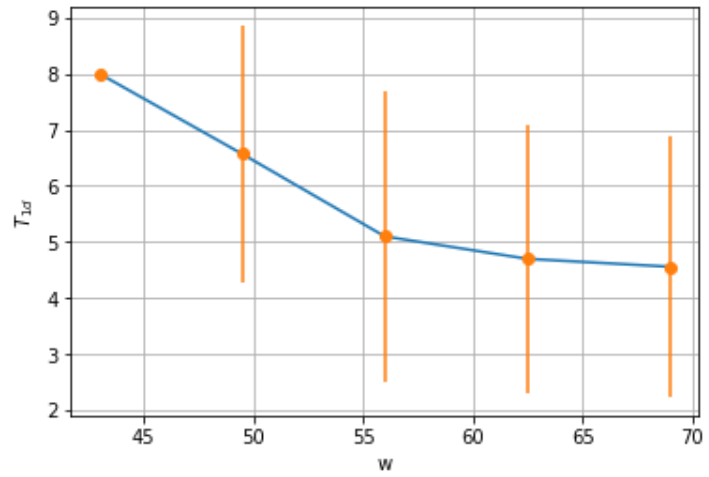
\includegraphics[width=1.0\linewidth]{diagram3a.jpg}
    \caption{コース幅 $w$ と$T_{\rm 1d}$の関係}
    \label{dia1}
\end{figure}
\vspace{-5mm}
\begin{figure}[!ht]
    \centering
    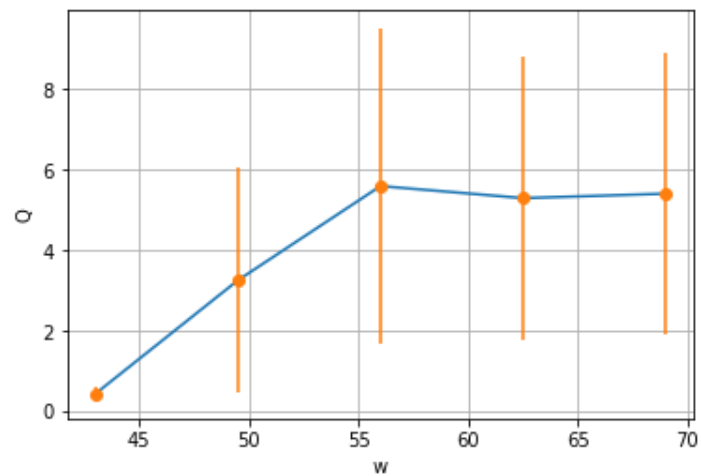
\includegraphics[width=1.0\linewidth]{diagram4a.jpg}
    \caption{$Q$とコース幅の関係}
    \label{dia2}
\end{figure}

幅が狭すぎる(43$cm$)と,長時間の渋滞が発生したことを観測した,ロボット同士のすれ違い,方向転換ができず,1方向走行流の状態にならなかった.大渋滞なので,流量もほとんどない.49.5$cm$の場合,渋滞も発生したので,1方向走行流になる時間($T_{\rm 1d}$)も長かったが,ロボットが方向転換できたので,流量も多少増えた.56$cm$から渋滞の発生が急激に減少し,ロボットの方向転換もしやすくなり,$T_{\rm 1d}$が減少した.以降コース幅が拡大して,$T_{\rm 1d}$がだんだん減少していた.流量については,56$cm$まで平均流量が増えて,69$cm$まで流量に明らかな変化が見られなくなった.

